%%
\documentclass{mcmthesis}
\mcmsetup{
        CTeX = false,   % 使用 CTeX 套装时,设置为 true
        tcn = 2213962, 
        problem = E,
        sheet = true, 
        titleinsheet = true,
        keywordsinsheet = true,
        titlepage = false,
        abstract = false
        }
        
\usepackage{mathpazo} 
\usepackage{lipsum}
\usepackage{algorithm}
\usepackage{bm}
\usepackage{algorithmicx}
\usepackage{algorithmic}
\usepackage{cite}
\usepackage{float}
\usepackage{subfigure}
\usepackage{multicol}
\usepackage{pdfpages}
\usepackage{indentfirst}
\usepackage{tikz}
\usepackage{pgfplots}
\usepackage{hyperref}
\usepackage{lastpage}
\usepackage{enumitem}
\usepackage{siunitx}
\usepackage{amssymb}
\usepackage{pgfplots}
\usepackage{multirow}
\usepackage{microtype}
\usepackage{textcomp}
\usepackage{gensymb}
\usepackage{vwcol}  
\usepackage{tabulary}
\usepackage{supertabular}
\usepackage{pgf-pie}
\usepackage{tabu}
\usepackage{verbatim}
\usepackage{graphicx}
\usepackage{fitbox}
\usepackage{wrapfig}


\definecolor{color1}{RGB}{251, 238, 172}
\definecolor{color2}{RGB}{244, 209, 96}
\definecolor{color3}{RGB}{138, 196, 208}
\definecolor{color4}{RGB}{40, 82, 122}
\definecolor{color5}{RGB}{157, 83, 83}
\definecolor{color6}{RGB}{99, 38, 38}
\definecolor{darkblue}{rgb}{0.0, 0.0, 0.55}
\definecolor{darkgray}{rgb}{0.66, 0.66, 0.66}

\setlength{\headheight}{13.6pt}

\title{\textbf{Dynamic Forest \& Brighter Future}}
\begin{document}
\begin{abstract}

%1. Introduce the background of the problem and be aware of you assignment.
%%简要引入背景,清晰交代任务。
In recent years, with global warming and other climate changes, the concept of "carbon" has attracted widespread public attention. Low-carbon-emission products such as clear energy has prevailed a lot. However, in addition to reducing carbon emissions, carbon sequestration is also a powerful way to mitigate carbon dioxide. With an attempt to effectively increase the amount of carbon sequestration and provide possible strategies for forest managers, our work is proceeded as follows.

%2. Point out the mathematical model you built, describe the purpose of your model and how it will be implemented.
%%指出你针对哪一任务,用了哪些模型、模型的目的以及实现的方法。
First of all, we establish a dynamic \textbf{SHG model} to simulate Sequestering-Harvesting-Growing carbon cycle of a forest ecosystem. A forest is divided into three parts: \textbf{product}, \textbf{mature} and \textbf{immature} area. They appear to be independent but influence each other. The model takes fixed parameters of the forest (area, tree species, region, etc.) as input and outputs the total amount of carbon sequestered over a period of time. By the Monte Carlo method, we obtain a haversting rate of \textbf{3\% to 5\% }that maximizes carbon sequestration.

%3. Give specific answers in the order of the questions.
%%每一步建模任务中,要依照问题顺序给出具体解答数字。
Secondly, we devise a comprehensive and practical indicator system, on which the \textbf{ECC model} is based. ECC model provides a value quantitative method in which we divide the values of forests into three categories: \textbf{ecological}, \textbf{economic} and \textbf{cultural} values. Among these, ecological value depends on the result of SHG model.

%4. Sensitivity and robustness analysis, possible model improvement.(if possible)
%%灵敏度、鲁棒性分析以及模型改进的可能。
Thirdly, according to the result of ECC model, we develop Target Oriented Forest Management Strategy by adopting \textbf{decision tree algorithm}. With 2,214 forest samples, we calculate the percentage of different values and put them as features into the algorithm, which automatically generates a decision tree with threshold. The final decision threshold value is \textbf{10.8\%} of economic value percentage and \textbf{69.5\%} of ecological value percentage. They can be viewed as a transition point in forest management. Forest managers can assess the current state of forest by calculating the combination of different values and compare it with the threshold to determine the future development directions. 

Finally, we apply our models in Heolongjiang Province of China and obtain the total 100-year carbon sequestration of $\bm{7.599\times 10^9}$ tonnes. During 2010 to 2018, the total value of it reaches to \textbf{92.2249} billion dollars in 2018 where ecological, economic and cultural value account for \textbf{81.64\%}, \textbf{12.68\%} and \textbf{5.67\%} respectively. According to our strategy, forests of Heilongjiang are in intermediate stage and they should adopt a culture-oriented strategy to develop tourism and enhance the input of scientific research. The transition point of management emerged in \textbf{2014-2015}. 

\begin{keywords}
Carbon Sequestration; SHG; Value Quantification; Decision-making
\end{keywords}
\end{abstract}
\maketitle

%% Generate the Table of Contents, if it's needed.
\tableofcontents
\newpage

\section{Assumptions and Justifications}
\begin{comment}
To simplify the problem, the following assumptions are made and justified.
\end{comment}

\begin{itemize}
  \item \textbf{Assumption 1:} The statistical data obtained are reliable and accurate.
	\begin{itemize}
  	 \item[$\hookrightarrow$] \textbf{Justification:} Most data are collected from authoritative websites and papers, under which our model is operational and practical.
 	\end{itemize}
  \item \textbf{Assumption 2:} The forest ecosystem is the smallest unit we consider.
        \begin{itemize} 
          \item[$\hookrightarrow$] \textbf{Justification:} Forest ecosystems are incredibly complicated. To preserve the macroscopic nature of the model, all data are collected on the principle that we view the forest as a whole.
        \end{itemize}
  \item \textbf{Assumption 3:} No massive unlawful logging activity will be carried out during the managing process, and the timber harvesting processes are all within control.
        \begin{itemize}
          \item[$\hookrightarrow$] \textbf{Justification:} During the regulating process, the executors will strictly stick to the plan, and the security of the forest resources can be guaranteed, which means there will not be any massive illegal timber harvesting process.
        \end{itemize}
  \item \textbf{Assumption 4:} Extreme events are ignored, which means fixed parameters are stable, such as the area of the forest, the structure of forest product, etc.
        \begin{itemize}
          \item[$\hookrightarrow$] \textbf{Justification:} Since the forest is stationary, we assume the biosphere is stable and developing. The force majeure will not be considered. 
        \end{itemize}
\end{itemize}
%第一章:简介
%主要包括:问题背景、问题复述、解决方案

\section{Assumptions and Justifications}
\begin{comment}
To simplify the problem, the following assumptions are made and justified.
\end{comment}

\begin{itemize}
  \item \textbf{Assumption 1:} The statistical data obtained are reliable and accurate.
	\begin{itemize}
  	 \item[$\hookrightarrow$] \textbf{Justification:} Most data are collected from authoritative websites and papers, under which our model is operational and practical.
 	\end{itemize}
  \item \textbf{Assumption 2:} The forest ecosystem is the smallest unit we consider.
        \begin{itemize} 
          \item[$\hookrightarrow$] \textbf{Justification:} Forest ecosystems are incredibly complicated. To preserve the macroscopic nature of the model, all data are collected on the principle that we view the forest as a whole.
        \end{itemize}
  \item \textbf{Assumption 3:} No massive unlawful logging activity will be carried out during the managing process, and the timber harvesting processes are all within control.
        \begin{itemize}
          \item[$\hookrightarrow$] \textbf{Justification:} During the regulating process, the executors will strictly stick to the plan, and the security of the forest resources can be guaranteed, which means there will not be any massive illegal timber harvesting process.
        \end{itemize}
  \item \textbf{Assumption 4:} Extreme events are ignored, which means fixed parameters are stable, such as the area of the forest, the structure of forest product, etc.
        \begin{itemize}
          \item[$\hookrightarrow$] \textbf{Justification:} Since the forest is stationary, we assume the biosphere is stable and developing. The force majeure will not be considered. 
        \end{itemize}
\end{itemize}
%第二章:模型假设
%主要包括:模型的假设

\section{Assumptions and Justifications}
\begin{comment}
To simplify the problem, the following assumptions are made and justified.
\end{comment}

\begin{itemize}
  \item \textbf{Assumption 1:} The statistical data obtained are reliable and accurate.
	\begin{itemize}
  	 \item[$\hookrightarrow$] \textbf{Justification:} Most data are collected from authoritative websites and papers, under which our model is operational and practical.
 	\end{itemize}
  \item \textbf{Assumption 2:} The forest ecosystem is the smallest unit we consider.
        \begin{itemize} 
          \item[$\hookrightarrow$] \textbf{Justification:} Forest ecosystems are incredibly complicated. To preserve the macroscopic nature of the model, all data are collected on the principle that we view the forest as a whole.
        \end{itemize}
  \item \textbf{Assumption 3:} No massive unlawful logging activity will be carried out during the managing process, and the timber harvesting processes are all within control.
        \begin{itemize}
          \item[$\hookrightarrow$] \textbf{Justification:} During the regulating process, the executors will strictly stick to the plan, and the security of the forest resources can be guaranteed, which means there will not be any massive illegal timber harvesting process.
        \end{itemize}
  \item \textbf{Assumption 4:} Extreme events are ignored, which means fixed parameters are stable, such as the area of the forest, the structure of forest product, etc.
        \begin{itemize}
          \item[$\hookrightarrow$] \textbf{Justification:} Since the forest is stationary, we assume the biosphere is stable and developing. The force majeure will not be considered. 
        \end{itemize}
\end{itemize}
%第三章:模型准备
%主要包括:记号说明、数据收集、数据清洗,以及其他与数据相关的点

\section{Assumptions and Justifications}
\begin{comment}
To simplify the problem, the following assumptions are made and justified.
\end{comment}

\begin{itemize}
  \item \textbf{Assumption 1:} The statistical data obtained are reliable and accurate.
	\begin{itemize}
  	 \item[$\hookrightarrow$] \textbf{Justification:} Most data are collected from authoritative websites and papers, under which our model is operational and practical.
 	\end{itemize}
  \item \textbf{Assumption 2:} The forest ecosystem is the smallest unit we consider.
        \begin{itemize} 
          \item[$\hookrightarrow$] \textbf{Justification:} Forest ecosystems are incredibly complicated. To preserve the macroscopic nature of the model, all data are collected on the principle that we view the forest as a whole.
        \end{itemize}
  \item \textbf{Assumption 3:} No massive unlawful logging activity will be carried out during the managing process, and the timber harvesting processes are all within control.
        \begin{itemize}
          \item[$\hookrightarrow$] \textbf{Justification:} During the regulating process, the executors will strictly stick to the plan, and the security of the forest resources can be guaranteed, which means there will not be any massive illegal timber harvesting process.
        \end{itemize}
  \item \textbf{Assumption 4:} Extreme events are ignored, which means fixed parameters are stable, such as the area of the forest, the structure of forest product, etc.
        \begin{itemize}
          \item[$\hookrightarrow$] \textbf{Justification:} Since the forest is stationary, we assume the biosphere is stable and developing. The force majeure will not be considered. 
        \end{itemize}
\end{itemize}
%第四章:模型一建立与求解
%主要包括:模型一的一些实现过程、模型一的结果(对问题的解答)

\section{Assumptions and Justifications}
\begin{comment}
To simplify the problem, the following assumptions are made and justified.
\end{comment}

\begin{itemize}
  \item \textbf{Assumption 1:} The statistical data obtained are reliable and accurate.
	\begin{itemize}
  	 \item[$\hookrightarrow$] \textbf{Justification:} Most data are collected from authoritative websites and papers, under which our model is operational and practical.
 	\end{itemize}
  \item \textbf{Assumption 2:} The forest ecosystem is the smallest unit we consider.
        \begin{itemize} 
          \item[$\hookrightarrow$] \textbf{Justification:} Forest ecosystems are incredibly complicated. To preserve the macroscopic nature of the model, all data are collected on the principle that we view the forest as a whole.
        \end{itemize}
  \item \textbf{Assumption 3:} No massive unlawful logging activity will be carried out during the managing process, and the timber harvesting processes are all within control.
        \begin{itemize}
          \item[$\hookrightarrow$] \textbf{Justification:} During the regulating process, the executors will strictly stick to the plan, and the security of the forest resources can be guaranteed, which means there will not be any massive illegal timber harvesting process.
        \end{itemize}
  \item \textbf{Assumption 4:} Extreme events are ignored, which means fixed parameters are stable, such as the area of the forest, the structure of forest product, etc.
        \begin{itemize}
          \item[$\hookrightarrow$] \textbf{Justification:} Since the forest is stationary, we assume the biosphere is stable and developing. The force majeure will not be considered. 
        \end{itemize}
\end{itemize}
%第五章:模型二建立与求解
%主要包括:模型儿的一些实现过程、模型二的结果(对问题的解答)

\section{Assumptions and Justifications}
\begin{comment}
To simplify the problem, the following assumptions are made and justified.
\end{comment}

\begin{itemize}
  \item \textbf{Assumption 1:} The statistical data obtained are reliable and accurate.
	\begin{itemize}
  	 \item[$\hookrightarrow$] \textbf{Justification:} Most data are collected from authoritative websites and papers, under which our model is operational and practical.
 	\end{itemize}
  \item \textbf{Assumption 2:} The forest ecosystem is the smallest unit we consider.
        \begin{itemize} 
          \item[$\hookrightarrow$] \textbf{Justification:} Forest ecosystems are incredibly complicated. To preserve the macroscopic nature of the model, all data are collected on the principle that we view the forest as a whole.
        \end{itemize}
  \item \textbf{Assumption 3:} No massive unlawful logging activity will be carried out during the managing process, and the timber harvesting processes are all within control.
        \begin{itemize}
          \item[$\hookrightarrow$] \textbf{Justification:} During the regulating process, the executors will strictly stick to the plan, and the security of the forest resources can be guaranteed, which means there will not be any massive illegal timber harvesting process.
        \end{itemize}
  \item \textbf{Assumption 4:} Extreme events are ignored, which means fixed parameters are stable, such as the area of the forest, the structure of forest product, etc.
        \begin{itemize}
          \item[$\hookrightarrow$] \textbf{Justification:} Since the forest is stationary, we assume the biosphere is stable and developing. The force majeure will not be considered. 
        \end{itemize}
\end{itemize}
%第六章:模型三建立与求解
%主要包括:模型三的一些实现过程、模型三的结果(对问题的解答)

\section{Assumptions and Justifications}
\begin{comment}
To simplify the problem, the following assumptions are made and justified.
\end{comment}

\begin{itemize}
  \item \textbf{Assumption 1:} The statistical data obtained are reliable and accurate.
	\begin{itemize}
  	 \item[$\hookrightarrow$] \textbf{Justification:} Most data are collected from authoritative websites and papers, under which our model is operational and practical.
 	\end{itemize}
  \item \textbf{Assumption 2:} The forest ecosystem is the smallest unit we consider.
        \begin{itemize} 
          \item[$\hookrightarrow$] \textbf{Justification:} Forest ecosystems are incredibly complicated. To preserve the macroscopic nature of the model, all data are collected on the principle that we view the forest as a whole.
        \end{itemize}
  \item \textbf{Assumption 3:} No massive unlawful logging activity will be carried out during the managing process, and the timber harvesting processes are all within control.
        \begin{itemize}
          \item[$\hookrightarrow$] \textbf{Justification:} During the regulating process, the executors will strictly stick to the plan, and the security of the forest resources can be guaranteed, which means there will not be any massive illegal timber harvesting process.
        \end{itemize}
  \item \textbf{Assumption 4:} Extreme events are ignored, which means fixed parameters are stable, such as the area of the forest, the structure of forest product, etc.
        \begin{itemize}
          \item[$\hookrightarrow$] \textbf{Justification:} Since the forest is stationary, we assume the biosphere is stable and developing. The force majeure will not be considered. 
        \end{itemize}
\end{itemize}
%第七章:模型检验
%主要包括:灵敏性检验、鲁棒性检验

\section{Assumptions and Justifications}
\begin{comment}
To simplify the problem, the following assumptions are made and justified.
\end{comment}

\begin{itemize}
  \item \textbf{Assumption 1:} The statistical data obtained are reliable and accurate.
	\begin{itemize}
  	 \item[$\hookrightarrow$] \textbf{Justification:} Most data are collected from authoritative websites and papers, under which our model is operational and practical.
 	\end{itemize}
  \item \textbf{Assumption 2:} The forest ecosystem is the smallest unit we consider.
        \begin{itemize} 
          \item[$\hookrightarrow$] \textbf{Justification:} Forest ecosystems are incredibly complicated. To preserve the macroscopic nature of the model, all data are collected on the principle that we view the forest as a whole.
        \end{itemize}
  \item \textbf{Assumption 3:} No massive unlawful logging activity will be carried out during the managing process, and the timber harvesting processes are all within control.
        \begin{itemize}
          \item[$\hookrightarrow$] \textbf{Justification:} During the regulating process, the executors will strictly stick to the plan, and the security of the forest resources can be guaranteed, which means there will not be any massive illegal timber harvesting process.
        \end{itemize}
  \item \textbf{Assumption 4:} Extreme events are ignored, which means fixed parameters are stable, such as the area of the forest, the structure of forest product, etc.
        \begin{itemize}
          \item[$\hookrightarrow$] \textbf{Justification:} Since the forest is stationary, we assume the biosphere is stable and developing. The force majeure will not be considered. 
        \end{itemize}
\end{itemize}
%第八章:结论
%主要包括:问题的解决方案
% \newpage
\section{Assumptions and Justifications}
\begin{comment}
To simplify the problem, the following assumptions are made and justified.
\end{comment}

\begin{itemize}
  \item \textbf{Assumption 1:} The statistical data obtained are reliable and accurate.
	\begin{itemize}
  	 \item[$\hookrightarrow$] \textbf{Justification:} Most data are collected from authoritative websites and papers, under which our model is operational and practical.
 	\end{itemize}
  \item \textbf{Assumption 2:} The forest ecosystem is the smallest unit we consider.
        \begin{itemize} 
          \item[$\hookrightarrow$] \textbf{Justification:} Forest ecosystems are incredibly complicated. To preserve the macroscopic nature of the model, all data are collected on the principle that we view the forest as a whole.
        \end{itemize}
  \item \textbf{Assumption 3:} No massive unlawful logging activity will be carried out during the managing process, and the timber harvesting processes are all within control.
        \begin{itemize}
          \item[$\hookrightarrow$] \textbf{Justification:} During the regulating process, the executors will strictly stick to the plan, and the security of the forest resources can be guaranteed, which means there will not be any massive illegal timber harvesting process.
        \end{itemize}
  \item \textbf{Assumption 4:} Extreme events are ignored, which means fixed parameters are stable, such as the area of the forest, the structure of forest product, etc.
        \begin{itemize}
          \item[$\hookrightarrow$] \textbf{Justification:} Since the forest is stationary, we assume the biosphere is stable and developing. The force majeure will not be considered. 
        \end{itemize}
\end{itemize}
%参考文献
\begin{appendices}
\vspace{-0.5cm}
\section{First appendix: Article for newspaper}

\newpage
\begin{figure}[H]
\centering
\setlength{\abovecaptionskip}{0.cm}
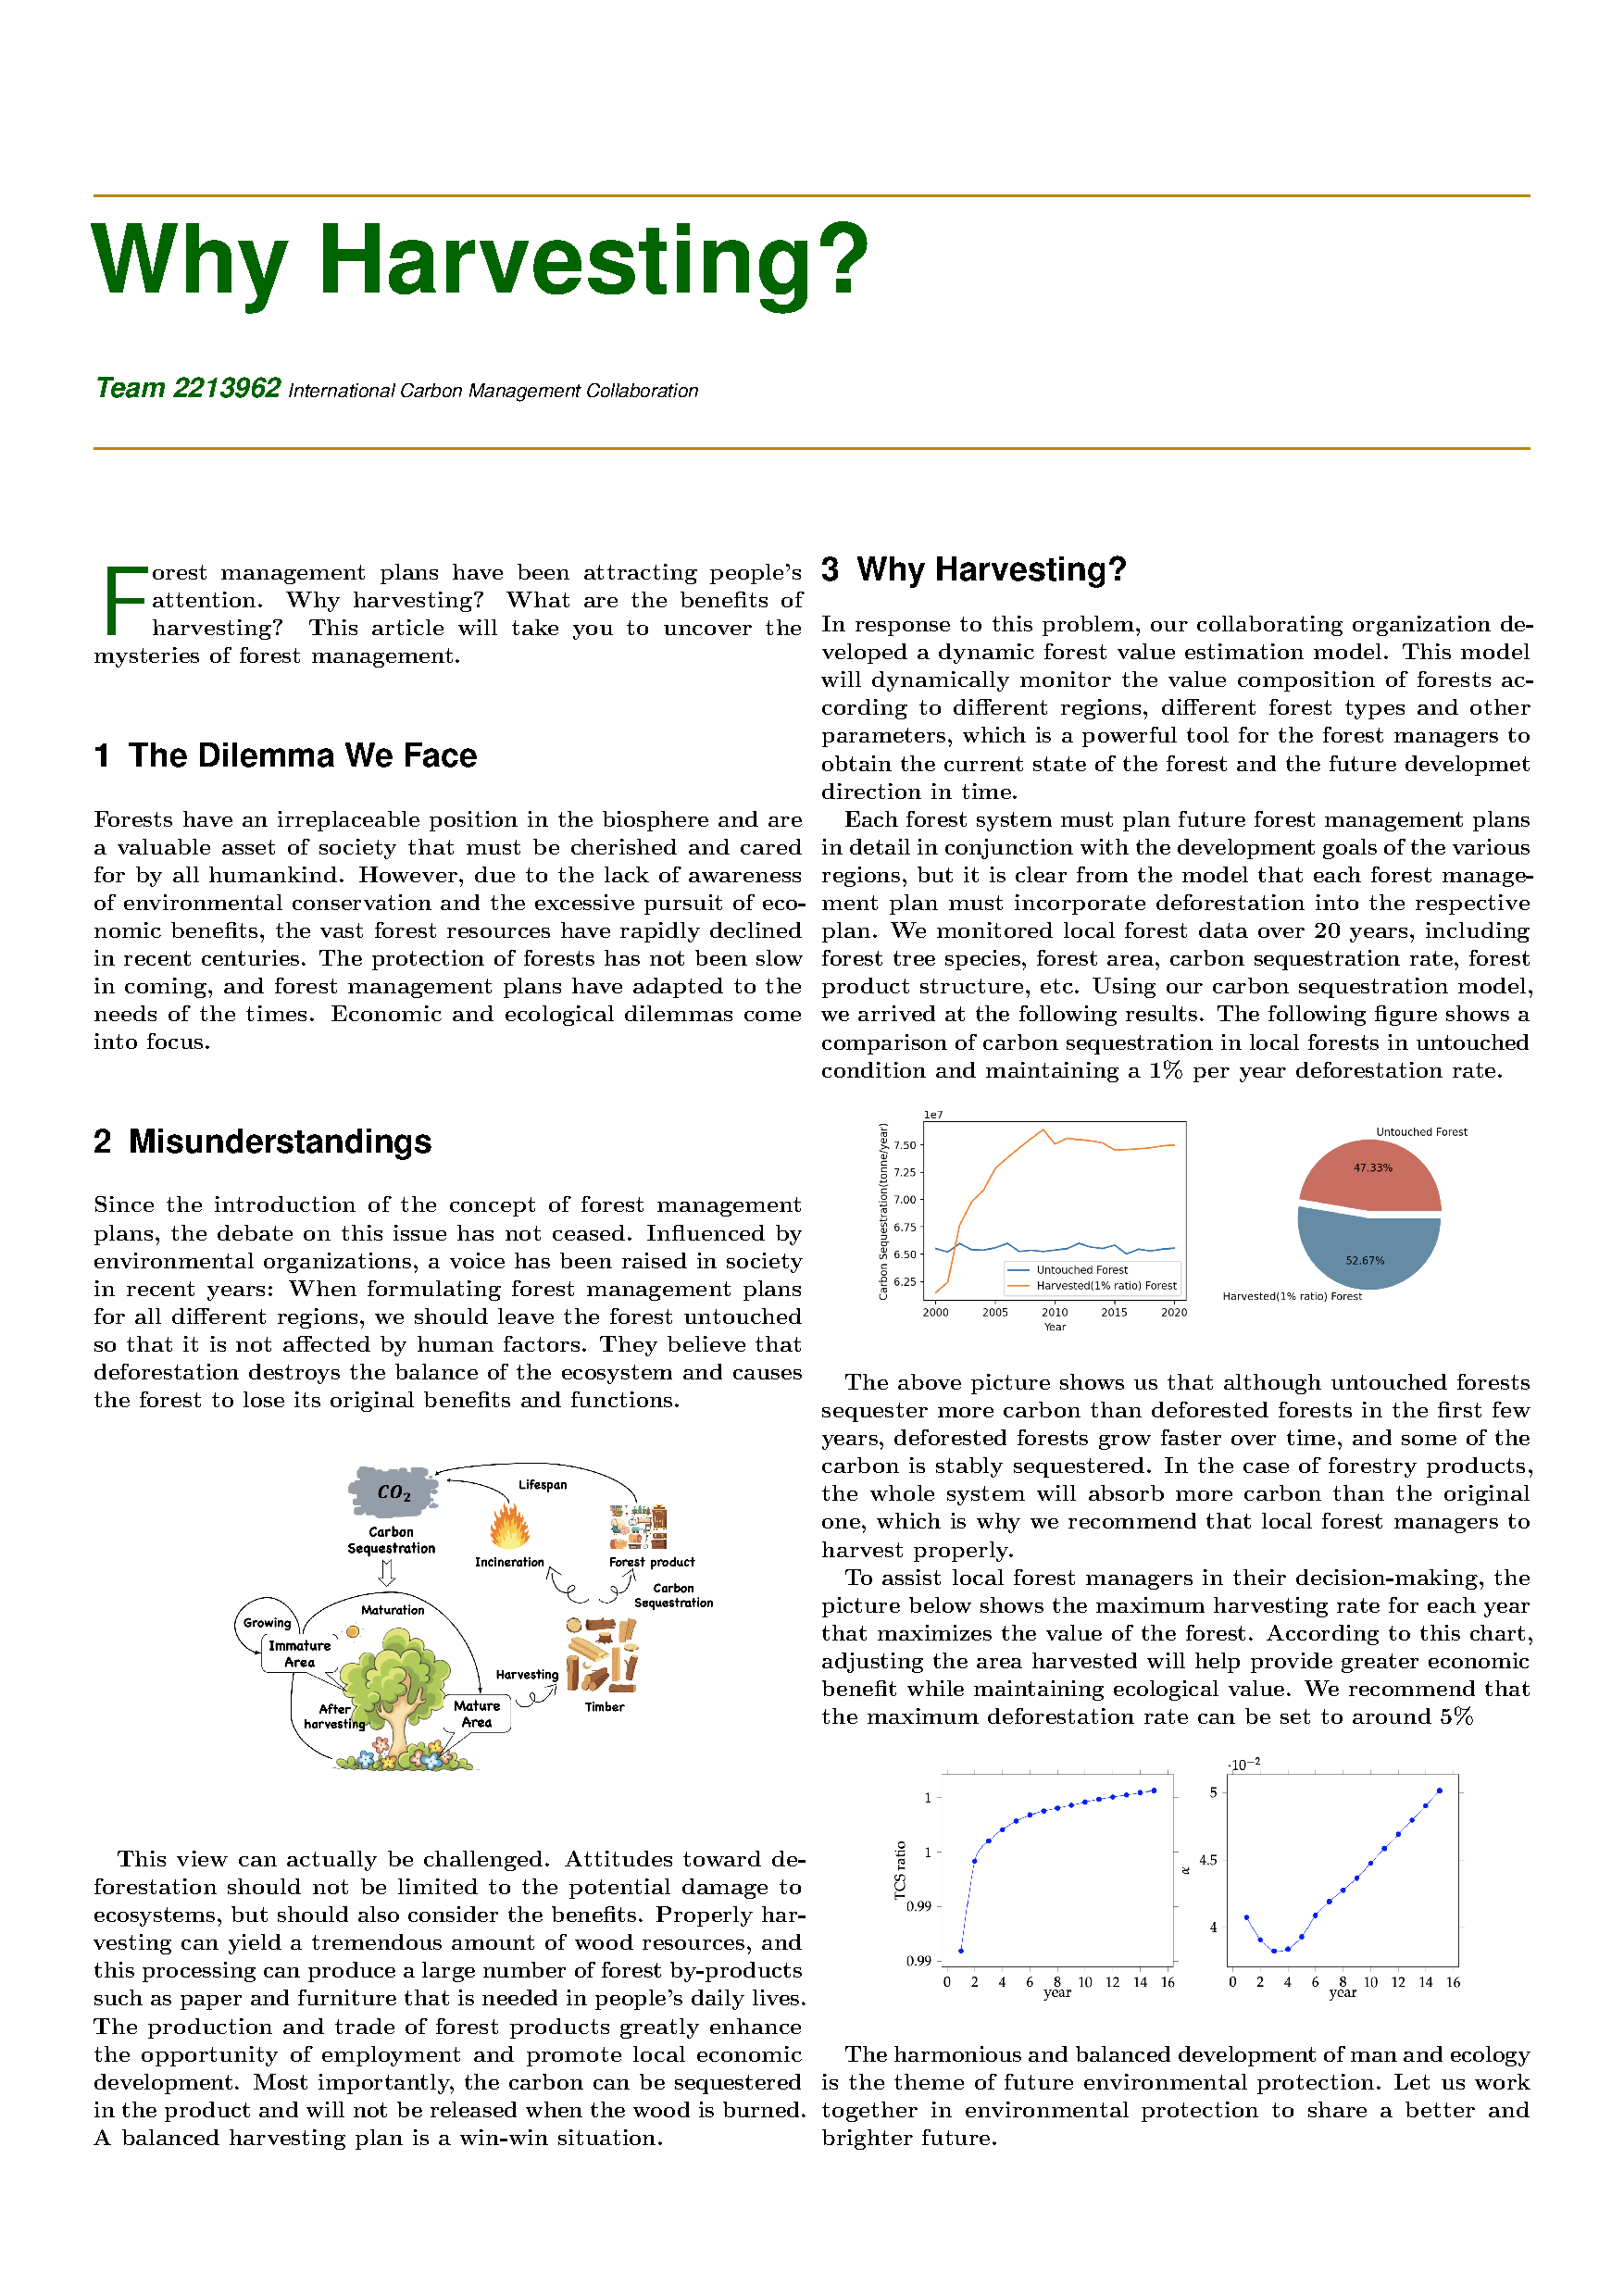
\includegraphics[width = \textwidth]{mcmthesis-demo/figures/Nontechnical Article.pdf}
\end{figure}
% \newpage

% \section{Second appendix: Ratio of wood products in different continents}

% \begin{table}[h]
% 	\centering
% %   \vspace*{-14cm}              % 调整图像上间距
% 	\caption{Ratio of wood products in different continents \cite{article}}
% 	\tabulinesep=1mm
% 	\begin{tabu}to \linewidth{X[c,m]X[2.5,c,m]X[c,m]X[c,m]X[c,m]X[c,m]X[c,m]X[c,m]}
% 		\tabucline[0.08em]-
% 		$i$ & $Item$                                  & $pp_{i, AF}$&  $pp_{i, AS}$ &  $pp_{i, EU}$ & $pp_{i, NA}$ & $pp_{i, Oce}$ & $pp_{i, SA}$\\ \tabucline[0.08em]-
% 		1	& Industrial roundwood                    & 10.95\%       &   0.1909\%            &     0.4947\%          &       0.5383\%       &     0.5998\%          &0.3604\%\\
% 		2	& Wood pellets and other agglomerates     & 0.0002\%	        &  0.0031\%             &    0.0262\%           &    0.0131\%          &  0.0029\%             &0.0113\%\\
% 		3	& Sawnwood                                & 0.0115\%	    &    0.0523\%           &     0.1256\%          &      0.0985\%        &   0.0898\%            &0.0588\%\\
% 		4	& Wood-based panel                        & 0.0021\%	        &   0.0393\%            &     0.0395\%          &    0.0372\%          &   0.0257\%            &0.0182\%\\
% 		5	& Papers                                  & 0.0141\%        &   0.1385\%            &     0.1836\%          &   0.2522\%           &      0.1373\%         &0.0918\%\\
% 		\tabucline[0.08em]-
% 	\end{tabu}
% %   \vspace*{-5mm}              % 调整图像下间距
%     \label{table}
% \end{table}

\end{appendices}
\end{document}
%% 
%% This work consists of these files mcmthesis.dtx,
%%                                   figures/ and
%%                                   code/,
%% and the derived files             mcmthesis.cls,
%%                                   mcmthesis-demo.tex,
%%                                   README,
%%                                   LICENSE,
%%                                   mcmthesis.pdf and
%%                                   mcmthesis-demo.pdf.
%%
%% End of file `mcmthesis-demo.tex'.

